\documentclass[xcolor=table]{beamer}

\usetheme[secheader,compress]{Madrid} %Primary theme

\usepackage{verbatim}
\usepackage{graphicx}
\usepackage{hyperref}

%% UTM Colors
\definecolor{UTMblue}{rgb}{0.043137, 0.137254, 0.254901}
\definecolor{UTMorange}{rgb}{1.0, 0.509803, 0}

\setbeamercolor{palette primary}{bg=UTMblue,fg=white}
\setbeamercolor{palette secondary}{bg=UTMblue,fg=white}
\setbeamercolor{palette tertiary}{bg=UTMblue,fg=white}
\setbeamercolor{palette quaternary}{bg=UTMblue,fg=white}
\setbeamercolor{structure}{fg=UTMblue} % itemize, enumerate, etc
\setbeamercolor{section in toc}{fg=UTMblue} % TOC sections
\setbeamercolor{title}{fg=UTMorange}

\setbeamercolor{subsection in head/foot}{bg=UTMorange,fg=white}

%%%%%%%%%%% BEGIN MACROS %%%%%%%%%%%%%%%%%%
% frameT: Frame with title
\newcommand{\frameT}[2]{\frame{\frametitle{#1} #2}}

% frameF: Fragile frame with title
\newcommand{\frameF}[2]{
  \begin{frame}[fragile]
    \frametitle{#1}
    #2
  \end{frame}
}

% frameTop: Frame aligned t the top
\newcommand{\frameTop}[2]{\frame[t]{\frametitle{#1} #2}}


\newcommand{\tab}{\hspace{1cm}}

\newcommand{\spaceor}{\hspace{5pt} \textbf{or} \hspace{5pt}}

%%%%%%%%%%% END MACROS %%%%%%%%%%%%%%%%%%%%



\begin{document}

\title{Senior Design Project - ParkSense}

\author{Aaron Alden, Spencer Karpati, Zachary Rose}
\institute{UT-Martin}
\date{\today}

%%%%%%%%%%% BEGIN TITLE %%%%%%%%%%%%%%%%%%
\frame{\titlepage}

%\section{Outline}
%%%%%%%%%%%% END TITLE  %%%%%%%%%%%%%%%%%%


\section{Introduction}
\frameT{Motivation} {
  Background
  \bigskip
  \begin{enumerate}
  \item Parking shortage
    \bigskip
  \item Computer Vision
    \bigskip
  \end{enumerate}

  \bigskip

}

%\frameT{Project Goals} {
% Described what you are trying to accomplish, including ``stretch'' goals.
%}

%\section{Sections--a useful organizational tool.}
\section{}

\frameT{Technology}{
  \begin{enumerate}
  \item Computer Vision and Machine Learning
    \begin{enumerate}
    \item OpenCV
      \bigskip
    \item Ultralytics: YOLOv8
    \end{enumerate}
    \bigskip
  \item Hardware
    \begin{enumerate}
    \item Raspberry Pi 2 Model B
      \bigskip
    \item Raspberry Pi Camera Module
    \end{enumerate}
  \end{enumerate}

}


\frameT{Demonstration}{
  \centering
  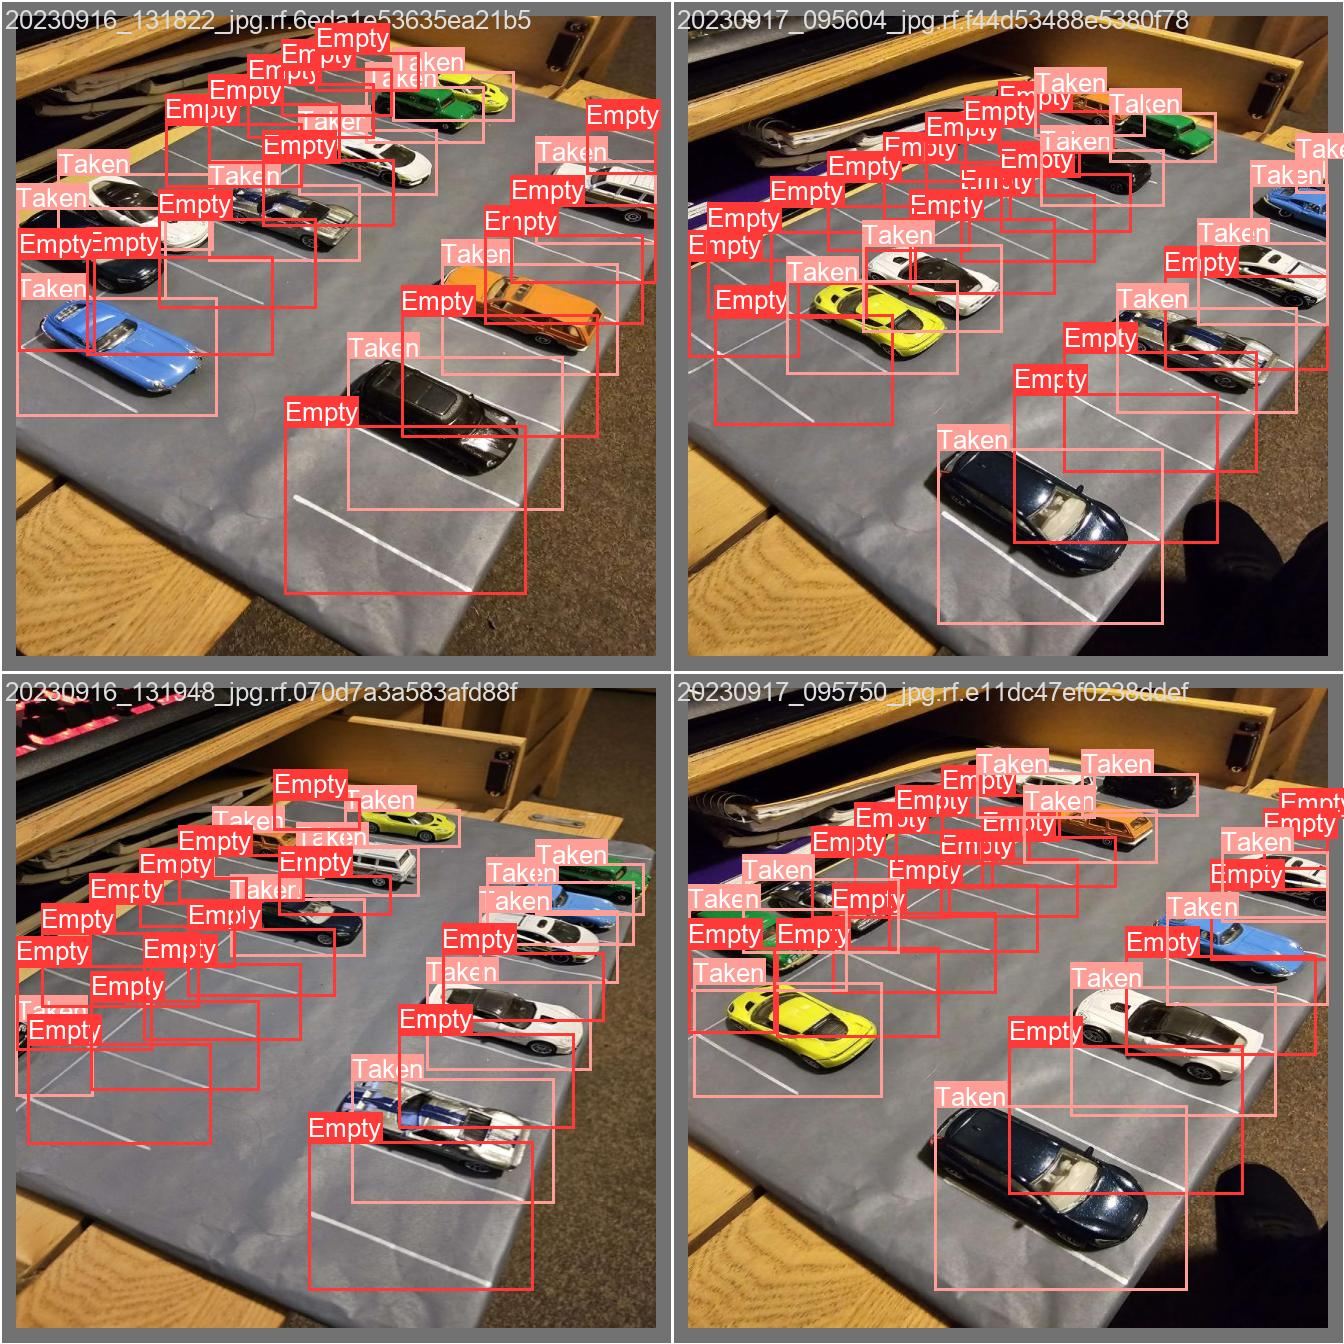
\includegraphics[width=.6\linewidth]{figures/CV_example.jpg}

  \href{https://spencek7746.github.io/Senior-Design-Project}{Webpage}
}

%\begin{frame}[fragile]
%\frametitle{Family Tree Knowledge Base}
%Facts:
%\begin{verbatim}
%Verbatim is a great way of enumerating code/algorithmic ideas.
%\end{verbatim}
%\end{frame}


%\frameT{How to include images} {
%% \includegraphics[width=.7\linewidth]{figures/image.pdf}
%}


%\begin{frame}[fragile]
%  \frametitle{Social Network Graph}
%  \begin{figure}[ht]
%    \begin{minipage}[b]{0.53\linewidth}
%      \centering
%      Minipages are a great way to
%    \end{minipage}
%    \hspace{0.5cm}
%    \begin{minipage}[b]{0.4\linewidth}
%      \centering
%      Line up side-by-side content.

%    \end{minipage}
%  \end{figure}

%\end{frame}


%\frameT{Results} {
%  Describe any results of your work here.

%  \bigskip

%  Things that worked?

%  \bigskip

%  Things that didn't work?
%}

%\frameT{Conclusions} {
%  Some bullet points here to wrap things up.
%}

\frameT{Any Questions?} {

  \begin{center}
    Questions?
  \end{center}
  \begin{center}
    Comments?
  \end{center}

  \bigskip

  Further project/author information:
  \begin{center}
    Please see our Github repo: \href{https://github.com/Spencek7746/Senior-Design-Project}{https://github.com/Spencek7746/Senior-Design-Project}
  \end{center}
  \begin{center}
    
\includegraphics[width=4cm]{figures/6AnLddq.png}
  \end{center}
}

%\frameF{fragile test} {
%}

%% \frameF{Prolog Family Tree} {
%% \begin{verbatim}
%% hello
%% \end{verbatim}



%% }

%Empty Page
%\frameT{Frame 1}{
%}


\end{document}
